\chapter{INTRODUÇÃO}
\begin{comment}
\begin{verbatim}
•	Contextualizar a proposta de trabalho no âmbito da empresa, de um outro trabalho já realizado, do ponto de vista científico e/ou tecnológico, etc.;
•	apresentar de forma clara os objetivos que se propõe atingir;
•	descrever de forma sucinta, mas objetiva, a solução preconizada ou a hipótese colocada;
•	apresentar de forma resumida, mas clara, os desenvolvimentos efetuados;
•	identificar como foi validada e avaliada a solução encontrada;
•	descrever a organização do relatório.
\end{verbatim}
\end{comment}
\section{CONTEXTUALIZÃO}
\begin{comment}
\begin{verbatim}
	Este projeto [7] surgiu do desejo de realizar um trabalho no âmbito da gestão de redes baseadas na infraestrutura Simple Network Management Protocol (SNMP) [4][5][8][9], mas que simultaneamente se integrasse na plataforma de alarmes do Sistema de Gestão de Alarmes (SGA) da Portugal Telecom (PT).
	Por coincidência, a PT tinha acabado de adquirir (à Alcatel) a nova rede de banda larga Internet Protocol (IP)—Multi Protocol Label Switching (MPLS), e assim surgiu a necessidade de integrar os alarmes gerados por esta infraestrutura (Figura 1) no SGA.
	
	
	Figura 1	Arquitetura do OSS 5620 SAM-O [1]
	Dada a pouca experiência, e conhecimento, sobre a aquisição de alarmes para este tipo de tecnologias, foi natural a proposta de incluir a integração, e tratamento, dos alarmes desta rede no âmbito do projeto. Esta inclusão refletiu-se no desenvolvimento de um processo de aquisição dos alarmes gerados e de um programa que formate os relatórios de alarme para o formato (normalizado) da notificação de alarme utilizado no SGA.
\end{verbatim}
\end{comment}
Num mundo altamente mecanizado, a força e o torque dentro de todas as grandezas são as quantidades mais medidas. Estas tem um papel significante nos produtos de medição de massa e células de peso usadas na industria e retalho, para os automóveis e aeronaves, no aperto de tampas de frascos de medicina e parafusos.\cite{book-9}\\
\\
A massa é uma das grandezas fundamentais, uma propriedade intrínseca de um objeto, na qual mede sua resistência a aceleração.
\begin{figure}[H]
	\centering
	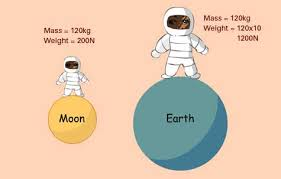
\includegraphics[height=7cm]{./image/PESTA/fisica/mass.jpg}
	\caption{Peso e Massa}
	\label{mass}
\end{figure}
Através da medição do peso, isto é, a força gravitacional exercida num dado objeto podemos calcular a massa. \cite{book-2}\\
\\
As balanças digitais estão presentes no nosso dia a dia, são uma ferramenta indispensável na industria, comercio e laboratórios. Determinar a massa dos objetos é uma moeda de troca no comercio, e um pilar fundamental da física e seu desenvolvimentos. Existe uma demanda tanto da área comercial como industrial que empurra o desenvolvimento dos sensores para obter melhores resultados quanto a precisão e imunidade de influencias exteriores na medição das grandezas mencionadas.\\
\\
Devido a importância desta grandeza a massa, foi a razão de querer fazer este projeto e desenvolver uma balança digital para uso domestico usando os meios que estão disponíveis no mercado.
\newpage
\section{OBJECTIVOS}
\begin{comment}
\begin{verbatim}
	O objetivo principal deste projeto é a aquisição dos alarmes provenientes da rede IP/MPLS da Alcatel e a sua integração no sistema atualmente em uso na PT. Dada a complexidade inerente a este objetivo, sentiu-se a necessidade de o subdividir em múltiplas tarefas de realização mais simples, tais como:
	•	A reavaliação dos procedimentos de aquisição de alarmes;
	•	O estudo do protocolo SNMP, nomeadamente o conceito e implementação de traps;
	•	O funcionamento e configuração dos programas que suportam o processo de leitura, destacando-se o snmptrapd e o syslog-ng;
	•	O desenvolvimento do programa que formate os relatórios de alarme para o formato (normalizado) da notificação de alarme utilizado no SGA;
	•	O aperfeiçoamento e simplificação de processo de desenvolvimento dos formatadores.
\end{verbatim}
\end{comment}
O Objetivo principal deste projeto é fazer uma balança digital economicamente viável, usando os sensores e equipamentos disponíveis no mercado, para ter um produto útil fácil de se replicar.
\\
\\
Escolher o sensor adequado e meios de tratamento da informação e comunicação vai ser o objeto de estudo. Tendo relevo ser um \textit{Embeded System} e utilizar as ferramentas necessárias para o executar.
\\
\\
No fim tentar aperfeiçoar, fazer melhorias, alterações e adaptações que possam surgir.
\newpage
\section{CALENDERIZAÇÃO}
O segundo semestre teve inicio em 8 de Março, num ambiente de pandemia COVID-19 onde fomos forçados ao ensinamento a distancia, todo o trabalho teve de ser acompanhado \textit{online} pelos docentes, no entanto tive de organizar as tarefas pretendidas no plano abaixo descrito.
\begin{comment}
\begin{verbatim}
	Sendo a aquisição dos alarmes provenientes da rede Alcatel IP/MPLS a motivação deste trabalho, a sua prossecução conduziu à calendarização apresentada na Tabela 1. Esta inclui um conjunto de tarefas, como por exemplo: o estudo da documentação do fabricante (Alcatel) da rede IP/MPLS adquirida pela PT; a implementação do coletor de alarmes, inserindo-o no processo de Recolha e Tratamento de Alarmes (RETA) [6]; teste e validação da solução proposta.
\end{verbatim}
\end{comment}
%%%%%%%%%%%%%%%%%%%%%%%%%%%%%%%%%%%%%%%%%%%%%%%%%%%%%%%%%%%%%%%%
\begin{comment}
\begin{tikzpicture}
	\GanttHeader{\textwidth}{2ex}{4cm}{15}
	\Task{1}{Requirement analysis}{0}{3}
	\Task{2}{Devise an abstract}{0.5}{1}
	\Task{3}{Develop interfaces}{3}{3}
	\Task{4}{Adapt existing}{4.5}{3}
	\Task{5}{Implement and evaluate}{5}{4.5}
	\Task{6}{Specify Phase II design}{8}{3}
	\Task{7}{Prepare final report}{11}{1}
\end{tikzpicture}
\end{comment}
%%%%%%%%%%%%%%%%%%%%%%%%%%%%%%%%%%%%%%%%%%%%%%%%%%%%%%%%%%%%%%%%
\begin{figure}[H]
	\caption{Calendarização das tarefas}
	%\begin{sidewaysfigure}
	\begin{ganttchart}[vgrid, hgrid]{1}{20}
		\gantttitle{Março}{5} 
		\gantttitle{Abril}{5}
		\gantttitle{Maio}{5}
		\gantttitle{Juno}{5}\\
		\gantttitlelist{1,...,20}{1}\\
		%First Group
		\ganttgroup{Requisitos}{2}{10} \\
		\ganttbar{Material}{3}{5} \\
		\ganttbar{\textit{Template} LaTeX}{5}{10} \\
		\ganttbar{\textbf{IDE} \textit{Template}}{3}{10}\\
		%\ganttlink{elem0}{elem1}
		%\ganttlink{elem1}{elem2}
		%\ganttlink{elem2}{elem3}
		%\ganttmilestone{Milestone 1}{11}
		%Second Group
		\ganttgroup{Projecto}{3}{20} \\
		\ganttbar{Kit Desenvolvimento}{3}{4} \\
		\ganttbar{Montagen Mesa Sensor}{5}{7} \\%5 7
		\ganttbar{HX711 comunicação}{4}{10} \\%4 8
		\ganttbar{Programção e Ensaio}{4}{20}\\
		%\ganttlink{elem4}{elem5}
		%\ganttlink{elem5}{elem6}
		%\ganttlink{elem6}{elem7}
		%\ganttmilestone{Milestone 1}{11}
		%Third Group
		\ganttgroup{Relatório}{9}{20} \\
		\ganttbar{Literartura}{8}{12} \\
		\ganttbar{Analise Documentação}{9}{12} \\
		\ganttbar{Validação}{10}{12} \\
		\ganttbar{Execução}{10}{20}
		%\ganttlink{elem8}{elem9}
		%\ganttlink{elem9}{elem10}
		%\ganttlink{elem10}{elem11}
		%\ganttmilestone{Milestone 1}{11}
	\end{ganttchart}
	\label{gantt}
%\end{sidewaysfigure}
\end{figure}
\newpage
\section{ORGANIZAÇÃO DO RELATÓRIO}
No capítulo 1 é feita uma contextualização do trabalho realizado e do seu propósito face às necessidades do mundo atual.\\
\\
No capítulo 2 vai ser descrito uma breve historia da evolução das balanças, e depois um estudo da balança digital.
%%%%%%%%%%%%%%%%%%%%%%%%%%%%%%%%%%%%%%%%%%%%%%%%%%%%%%%%%%%%%%%%
\chapter{História da Balança}
%%%%%%%%%%%%%%%%%%%%%%%%%%%%%%%%%%%%%%%%%%%%%%%%%%%%%%%%%%%%%%%%
As balanças foram criadas por necessidade durante o desenvolvimento do comercio na antiguidade, os produtos que não recorriam a contagem por unidades, tais como objetos irregulares por exemplo o ouro tinha de se quantificar seu valor, e a forma de medir sua massa tornou-se numa variável de medição para a troca de bens.\\
\\
A relíquia mais antiga de uma balança de medir massa foi descoberto na vila de \textit{Indus River}, perto do conhecido por hoje de Pakistão, e estima-se ser por volta de \textcolor{blue}{2000} B.C.\\
Estas primeiras balanças eram alavancas em equilíbrio $[ \; F_{1} \times b_{1c} = F_{2} \times b_{2c} \; ]$, onde nos extremos eram colocados cestos e se colocava os pesos, este estava centrado no seu centro de massa, assim se os pesos nos dois cestos serem iguais fica em equilíbrio (na horizontal), era um sistema de comparar com pesos fixos estabelecidos como norma (\textbf{contra-pesos}).
\\
\begin{minipage}[!b]{0.45\linewidth}
	\begin{figure}[H]
		\centering
		\includegraphics[height=7cm]{./image/PESTA/general/balanca_1.jpg}
		\caption{Balança medieval}
		\label{balanca_1}
	\end{figure}
\end{minipage}
\hspace{2.2cm}
\begin{minipage}[!b]{0.45\linewidth}
	\begin{figure}[H]
		\centering
		\includegraphics[height=7cm]{./image/PESTA/general/balanca_4.jpg}
		\caption{Balança}
		%\caption{Balança moderna \cite{book-7}}
		\label{balanca_4}
	\end{figure}
\end{minipage}
\newline
\newline
\newline
Este sistema pode ter uma boa precisão, mas também pode se facilmente ser adulterado.
\\
\\
Os métodos de medir a massa de objetos não conheceu nenhumas melhorias tecnológicas relevantes até a era industrial. Só nos fins do século \textcolor{blue}{\textit{XVIII}} é que o meio de medir a massa de objetos não dependia de \textbf{contra-pesos}. As balanças por molas foi inventado por \textbf{\textit{Richard Salter}}, um fabricante de balanças por volta dos anos de \textcolor{blue}{1770} na Inglaterra.\\
\begin{figure}[H]
	\centering
	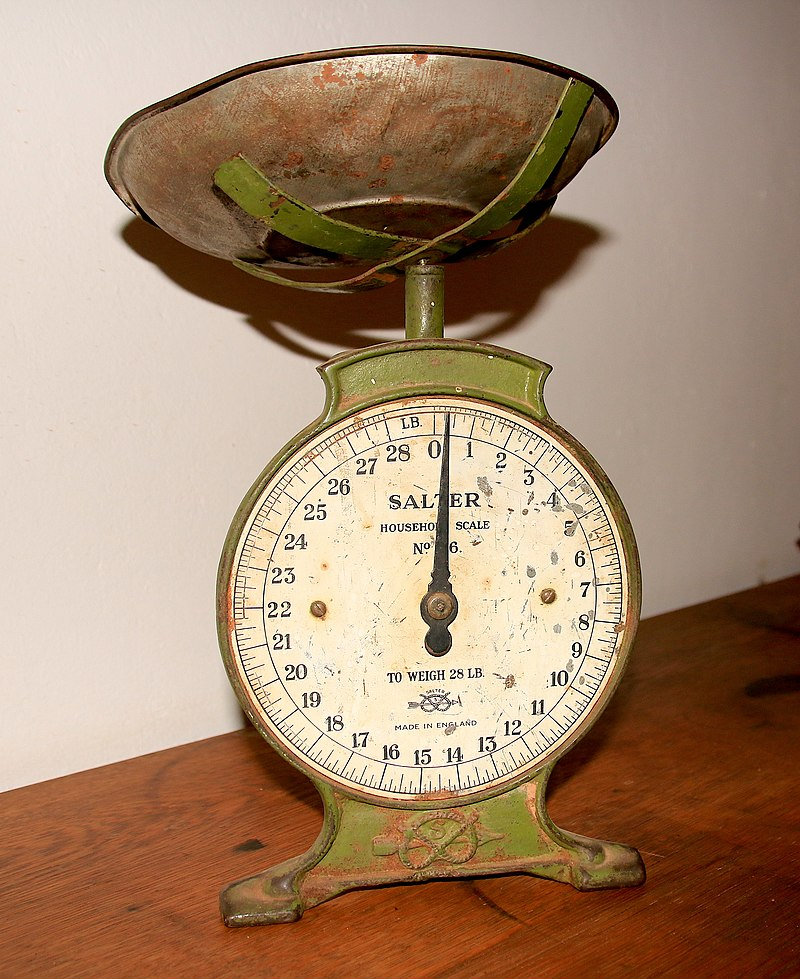
\includegraphics[height=7cm]{./image/PESTA/general/Weigh_Scale_Salter_1.jpg}
	\caption{Balança de Salter}
	\url{https://en.wikipedia.org/wiki/Salter_Housewares}
	\label{Weigh_Scale_Salter_1}
\end{figure}
A balança por mola, como o nome implica, mede a pressão (ou sua tensão) exercido sobre a mola para determinar a massa do objeto. Este tipo de balanças ainda são muito comum nos dias de hoje por serem bastante económicas de fabricar, mas não tem tanta precisão como as eletrónicas desenvolvidas e aperfeiçoadas durante o século \textcolor{blue}{\textit{XX}}.
\newline
\newline
\begin{minipage}[!b]{\linewidth}
	\begin{figure}[H]
		\captionsetup{justification=raggedright,singlelinecheck=false}
		\flushleft
		\includegraphics[height=7cm]{./image/PESTA/general/Public_Body_Scales_1.jpg}
		\hspace{.8cm}
		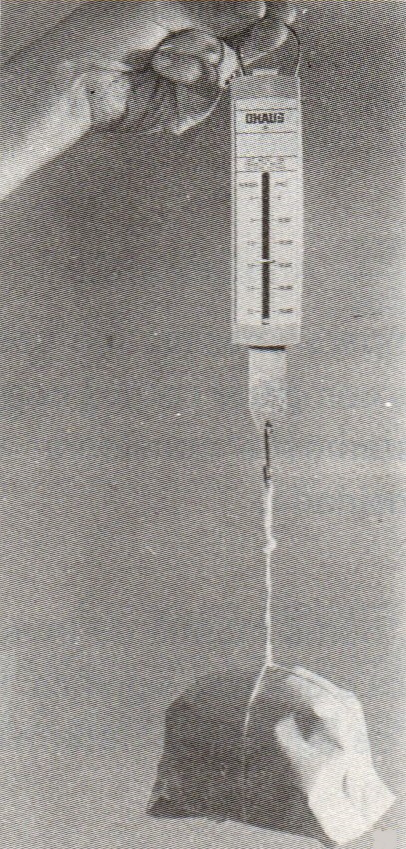
\includegraphics[height=7cm]{./image/PESTA/general/Balanca_Mola_1.jpg}
		\caption{Balanças de Mola}
		\label{Balanca_Mola_1}
	\end{figure}
\end{minipage}
\newpage
As balanças eletrónicas mais modernas utilizam resistências elétricas em materiais permeáveis e fazer passar uma corrente elétrica na qual é possível detetar a variação de condutividade das resistências em que é proporcional a pressão exercida sobre esse material, podendo dai se deduzir o peso dos objetos.
\begin{figure}[H]
	\centering
	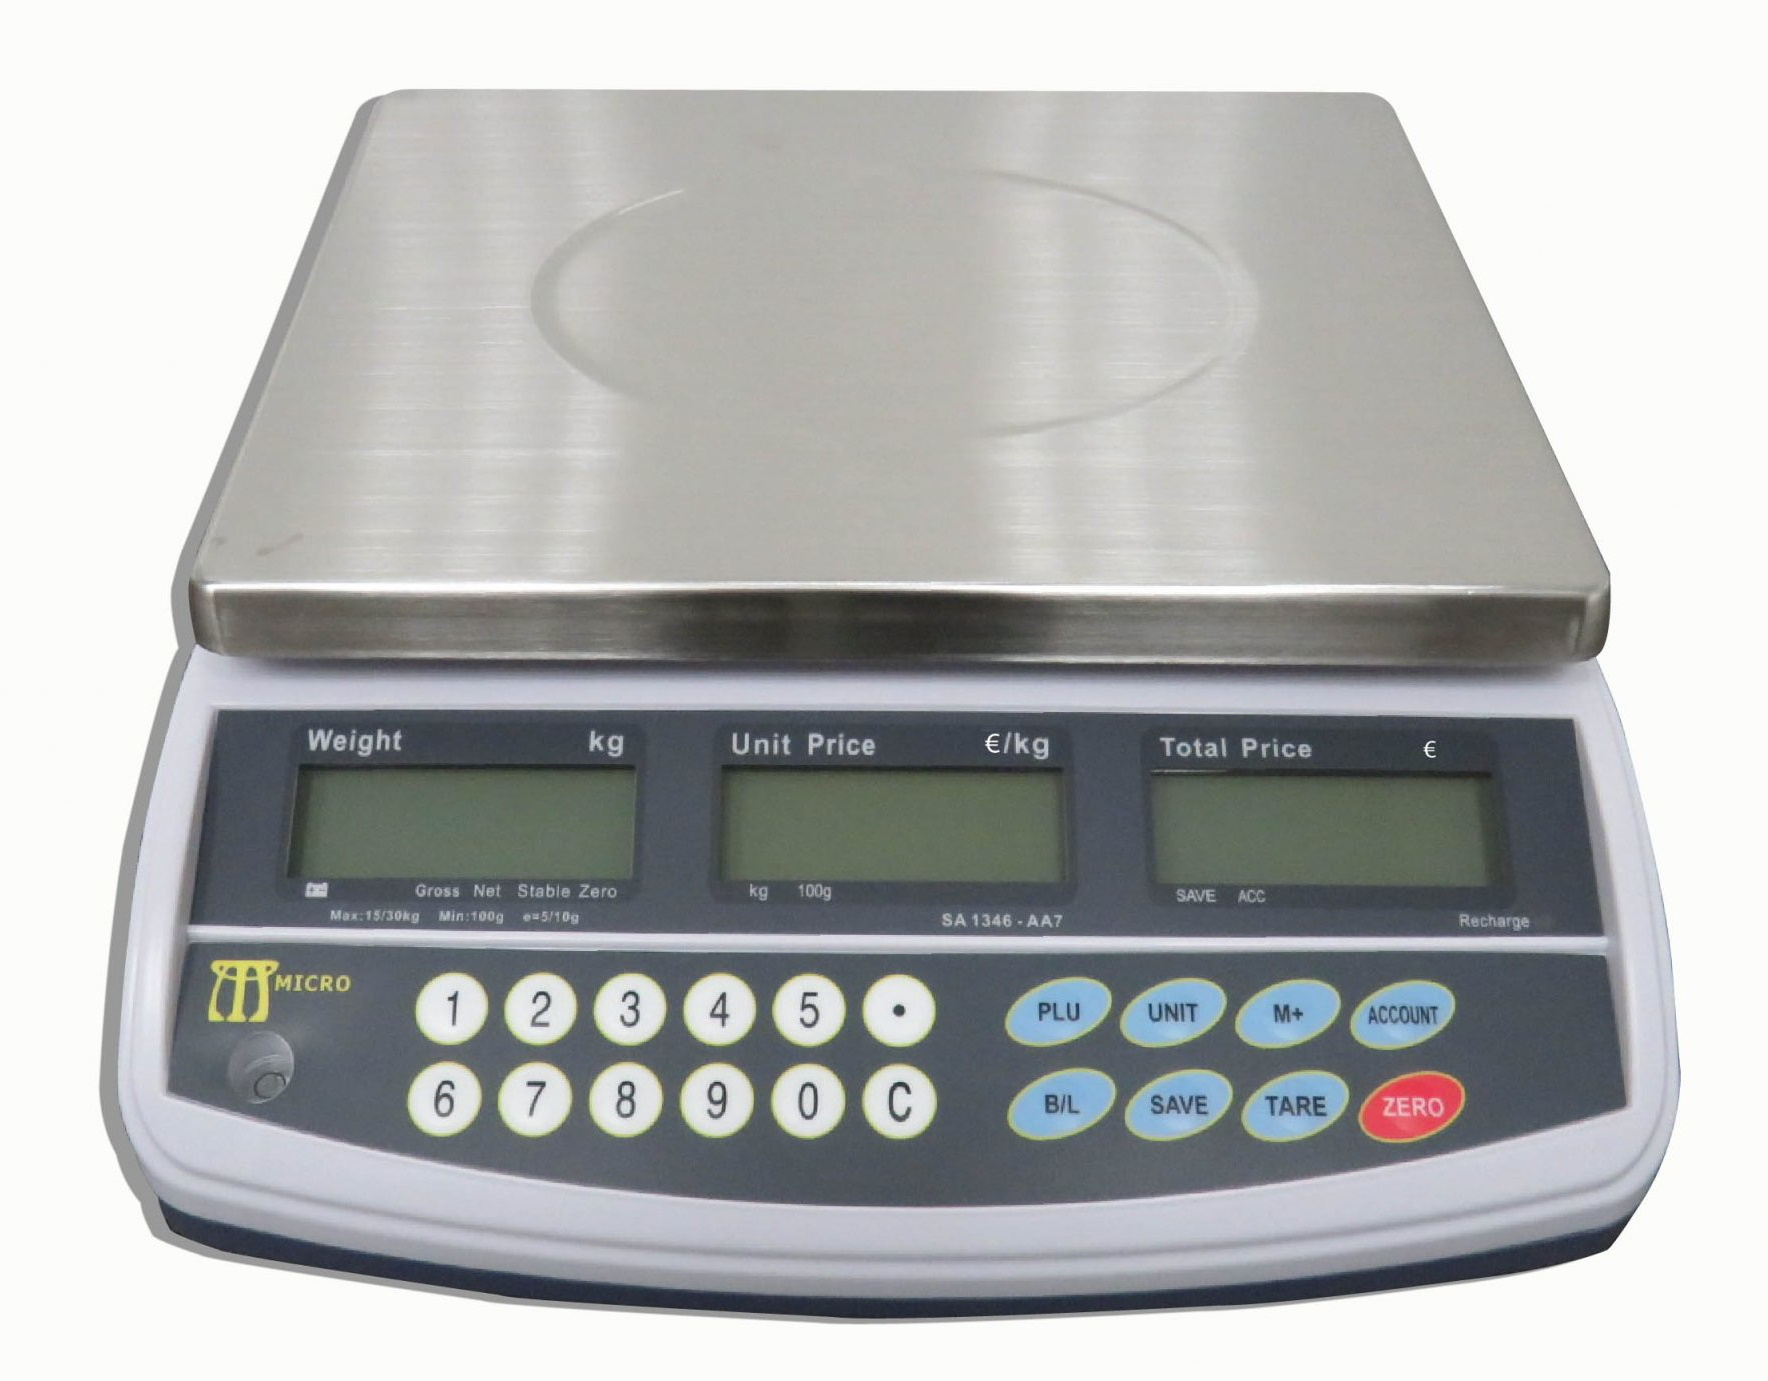
\includegraphics[height=7cm]{./image/PESTA/general/Scale_1.jpg}
	\caption{Balança eletrónica}
	\label{Scale_1}
\end{figure}
O que vai ser utilizado no projeto vai ser um \textbf{célula de peso} que seque o principio acima mencionado, estas células tem quatro sensores \textit{\textbf{strain gauges}} ligadas em ponte \textit{wheatstone} que vão detetar a distorção (pressão) do material, ou seja, a célula de peso e gerar um sinal em tensão proporcional a força exercida quando alimentada. Seque o mesmo principio de uma mola.
\begin{equation}
	\label{eq:Hooke}
	K = \frac{\Delta l}{F}
\end{equation}
Também há outros tipos de células de peso tais como as pneumáticas e hidráulicas que convertem a pressão num sinal elétrico que é proporcional a força nela exercida.
\begin{equation}
	\label{eq:Preasure}
	P = \frac{F}{A}
\end{equation}
As células de peso capacitivas são outro exemplo de como obter um sinal proporcional a força imposta como carga, neste caso é medido sua capacidade pelo afastamento ou aproximação dos pratos dos elétrodos.
\begin{equation}
	\label{eq:Capacity}
	C = \varepsilon_{0} \; \varepsilon_{r} \; \frac{A}{d}
\end{equation}
Pode-se dizer que em todos os casos determina-se a força resultante através do deslocamento no espaço.
\chapter{Balança Digital}
\section{Sensor}
Para medir a massa recorreu-se a uma \textbf{célula de peso} que determina a pressão exercida por um dado objeto, neste caso é um bloco de alumínio como indicado na \textit{figura} \ref{Load_Cell_1}, para isso ser possível este utiliza sensores Piezoresistivos numa montagem em ponte \textit{wheatstone} sobre essa superfície em locais determinados.
\begin{figure}[H]
	\captionsetup{justification=raggedright,singlelinecheck=false}
	\flushleft
	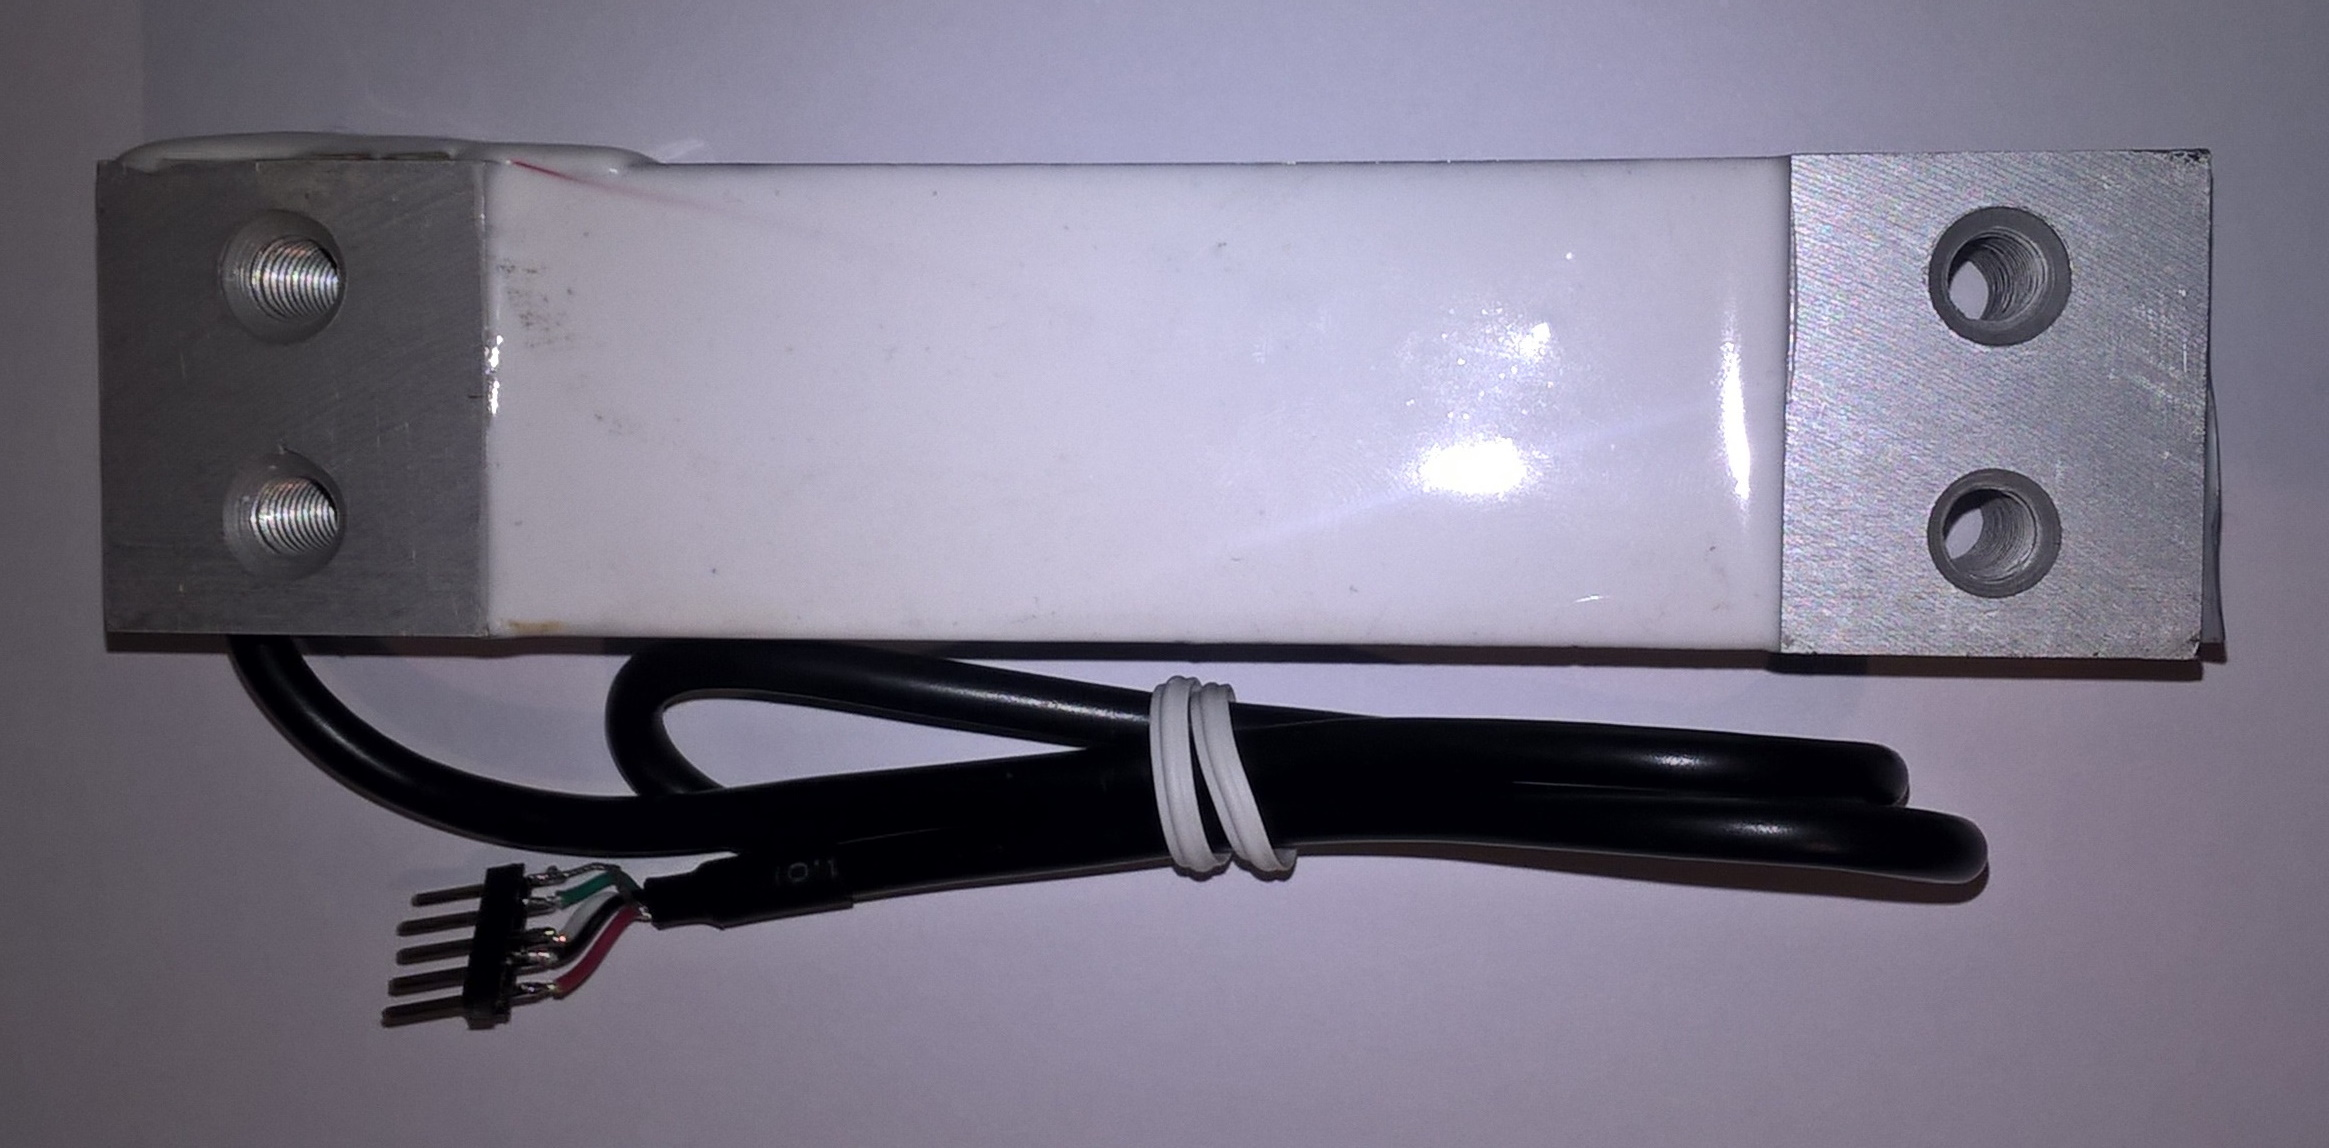
\includegraphics[scale=0.15]{./image/PESTA/material/Load_Cell_1.jpg}
	\caption{Célula de Peso 50Kg}
	\label{Load_Cell_1}
\end{figure}
Piezoresistividade deriva seu nome da palavra grega \textit{piezin}, que significa "pressionar". É um efeito exibido por vários materiais que exibem uma mudança na resistividade devido a uma pressão aplicada. O efeito foi descoberto pela primeira vez por Lord Kelvin em \textcolor{blue}{1856}, que notou que a resistência dos fios de cobre e ferro aumentava quando em tensão. Ele também observou que os fios de ferro apresentavam uma alteração maior na resistência do que os de cobre. A primeira aplicação do efeito piezoresistivo não apareceu até a década de \textcolor{blue}{1930}, cerca de \textcolor{blue}{75} anos após a descoberta de Lord Kelvin. Em vez de usar fios de metal, esses assim chamados medidores de tensão são geralmente feitos de uma folha de metal fina montada em uma película de suporte, que pode ser colada em uma superfície. O sensor de fita de metal típico é representado na \textit{figura} \ref{strain_gauge_1} \cite{book-9}
\begin{figure}[H]
	\centering
	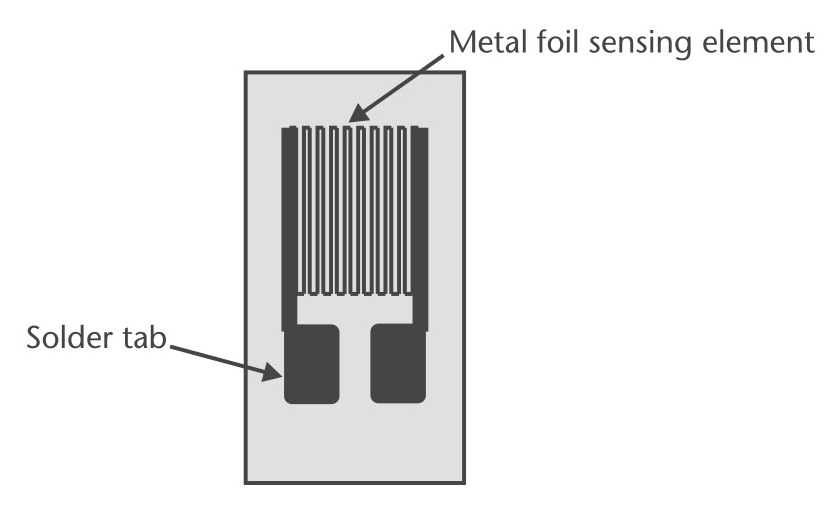
\includegraphics[height=5cm]{./image/PESTA/general/strain_gauge_1.jpg}
	\caption{Fita metálica \textit{strain gauge} \cite{book-9}}
	\label{strain_gauge_1}
\end{figure}
\section{Amplificador}
A amplificação é geralmente um requisito fundamental, pois a maioria dos sensores tende a produzir níveis de sinal significativamente mais baixos do que aqueles usados no processador digital. Sensores resistivos podem precisar de um amplificador de carga. Se possível, é vantajoso ter o ganho o mais próximo possível do elemento sensor. Em situações onde um alto ganho é necessário, muitas vezes pode haver implicações para lidar 
com quaisquer efeitos adversos, como o ruído, também em termos de \textit{layout} do \textit{chip}, os transitórios agudos associados aos sinais digitais precisam ser mantidos bem longe dos circuitos analógicos \textit{front-end}. \cite{book-9}
\section{Informação}
A conversão de informação é a transição entre o sinal continuo da vida real para um sinal discreto associado ao mundo digital, tipicamente esta etapa consiste na conversão analógica para digital.
\\
O processamento digital pode consistir de rotinas para compensar os desvios por linearização, compensação da sensibilidade e \textit{offset}, ou podem ser técnicas mais sofisticadas como reconhecimento de padrões (tais como redes neuronais) para equipamentos de sensores vetoriais.\cite{book-9}
\\
A comunicação trata de cuidar das rotinas necessárias para transferir e receber a informação e sinais de controle para a linha de comunicação com o sensor, e o processador toma lugar como componente central tratando a informação, guardar os dados e fazer rotinas tais como de calibração, teste e controlo de ganho da amplificação. \cite{book-9}
%%%%%%%%%%%%%%%%%%%%%%%%%%%%%%%%%%%%%%%%%%%%%%%%%%%%%%%%%%%%%%%%
\begin{comment}

Measurement devices need to be robust to withstand changing environmental influences such as temperature, vibration, and humidity, and they must also provide reliable measurement over long periods of time. Mechanical interfacing of the devices can be difficult and can influence final measurement. The forces and torques may change rapidly, and so the devices must have adequate frequency and transient responses.\\
There are several methods to measure forces and torques. Often, the force to be measured is converted into a change in length of a spring element. The change in dimensions is subsequently measured by a sensor, for example, a piezoresistive, a capacitive or a resonant sensor.\\
It is not so surprising, therefore, that most force and torque measurement devices utilize the long and well-established resistance strain gauge technology.\\
Unfortunately, the metallic resistance strain gauge is relatively insensitive such that in use it is normal to obtain only several millivolts of analog voltage before amplifi-
cation, and the gauges must not be significantly overstrained. The rangeability and overloading capabilities are seriously restricted. Also, the gauges consume relatively high electrical power (e.g., 250 mW).\\
In general, measurement instrumentation now needs smaller sensing devices of lower power consumption and with greater rangeability and overload capabilities.\\
Greater compatibility with digital microelectronics is highly desirable. Noncontact and wireless operation is sometimes needed, and in some cases batteryless devices
are desirable. Production of measurement devices using metallic resistance strain gauges can be relatively labor intensive and skilled, and may require relatively ineffi-cient calibration procedures.\\
In recent years some instrument manufacturers of force and torque measure-ment devices have moved away from using resistance strain gauges. Already, one leading manufacturer of weighing machines for retail and industrial applications
now uses metallic and quartz resonant tuning fork technologies, and smaller compa-nies have established niche markets using surface acoustic wave (SAW) technology, optical technology, and magnetoelastic technology.\\
Further commercial developments are taking place to enhance device manufacturability and improve device sensitivity and robustness in operation. Measurement on stiffer structures at much lower strain levels is now possible. The worldwide sen-
sor research base is very active in exploring MEMS for sensing force and torque, and the rest of this chapter will review the current situation and future prospects.\\
\\
The market pull provided by the automotive industry—for example,
for manifold air pressure sensors—has led to the development of successful devices and technologies that have benefited a wide range of other pressure sensing applica-tions.
\end{comment}